\documentclass[a4paper,11pt,]{article}
\usepackage{fancyvrb, color, graphbox, hyperref, amsmath, url}
\usepackage{palatino}
\usepackage{graphicx}
% \usepackage{pygments}
% \usepackage{minted}
\usepackage[a4paper,text={16.5cm,25.2cm},centering]{geometry}
\usepackage{lipsum}
\usepackage[labelformat=simple,position=top]{subcaption}
% \renewcommand\thesubfigure{\alph{subfigure})}
\hypersetup{
  pdfauthor = {Srdjan Sarikas},
  pdftitle={Intracellular Receptors},
  colorlinks=TRUE,
  linkcolor=blue,
  citecolor=red,
  urlcolor=green
}
\newcommand{\Regions}{{\texttt{Regions}}}

%\setlength{\parindent}{0pt}
%\setlength{\parskip}{1.2ex}

\title{Intracellular Receptors \\ {\small Materials and Methods: Analysis and Processing}}

\author{Srdjan}
\date{\today}

\begin{document}
\maketitle

%<<echo=False>>=
%import matplotlib.pyplot as plt
%import numpy as np
%import pandas as pd
%from islets import load_regions
%@

\section{General pipeline}

A typical experiment involving imaging of pancreatic slices in our lab concerns a single field of view
showing 10s--100s of cells, in a recording of at least several, often dozens, of gigabytes.
Current tools (ImageJ, \dots) rely on loading the recording, or its part, into memory, for viewing, analysis, and processing.
It also requires laborious and long human engagement.
We have developed a set of interdependent tools to automatize as much as possible the pipeline. 
The crucial elements of our pipeline are the following:
\begin{itemize}
\item (Semi-)automatic detection of regions of interest (ROIs);
\item Transformation of ROI time traces into standard score ("z-score");
\item Quantification of the phenotype for each ROI in terms of the distribution of events of different durations.
\end{itemize}

Our toolset is inspired and relies on CaImAn \cite{giovannucci2019caiman}, a similar package developed for the purposes in neuroscience research.

\begin{figure}[h]
\centering
\includegraphics[width=\textwidth,trim=1.5cm 1.5cm 15mm 15mm,clip]{figures/pipeline.pdf}
\label{fig:pipeline}
\caption{
An illustration of our processing and analysis pipeline:
({\it i})  From a full movie, we calculate the mean (or other statistic) across all frames.
({\it ii}) We pass the mean image through a band-pass filter and define ROIs by detecting local peaks.
({\it iii}) We save ROIs with all the important information (time traces, ROI coordinates, movie statistics, recording frequency, pixel size, etc.).
({\it iv}) Traces contain features at very different time scales---with different timescales presumably important for different cell types. We collect them into separable events for analysis.
}
\end{figure}

\subsection{(Semi-)Automatic Detection of Regions of Interest}

Once imported, a recording is stored as a 3-dimensional ($T{\times}x{\times}y$) numpy array \cite{2020NumPy-Array}.
When the recording is stable, obtaining a mean image, or any other statistic over frame, is rather trivial. 
In case there is horizontal movement, it can be corrected for by aligning the frames to a template. 
For this we use the functionality present in CaImAn \cite{giovannucci2019caiman}, except that high frequency recordings need to be rebinned to some moderate frequency (a few Hz), before correcting, in order to reduce the noise level. 
Once the translation offsets are obtained, we use them to correct the recording in original frequency.

To define regions of interest, we blur the representative image by a kernel of the size we expect cells to be, 
and at the scale double of that.
The difference between these two images represents a band-pass filter of the original, where the local intensity variation are emphasized (fig.\ref{fig:regions}).
We then pass through all pixels where the value of the filtered image is positive (or larger than a small positive threshold), and for each pixel we search for a local peak in its vicinity. 
All the pixels that lead to the same local peak are then grouped into a single ROI.


\begin{figure}[t]
\centering
\begin{minipage}{.25\textwidth}
    \vskip 2mm
    {\fontfamily{phv}\selectfont A} 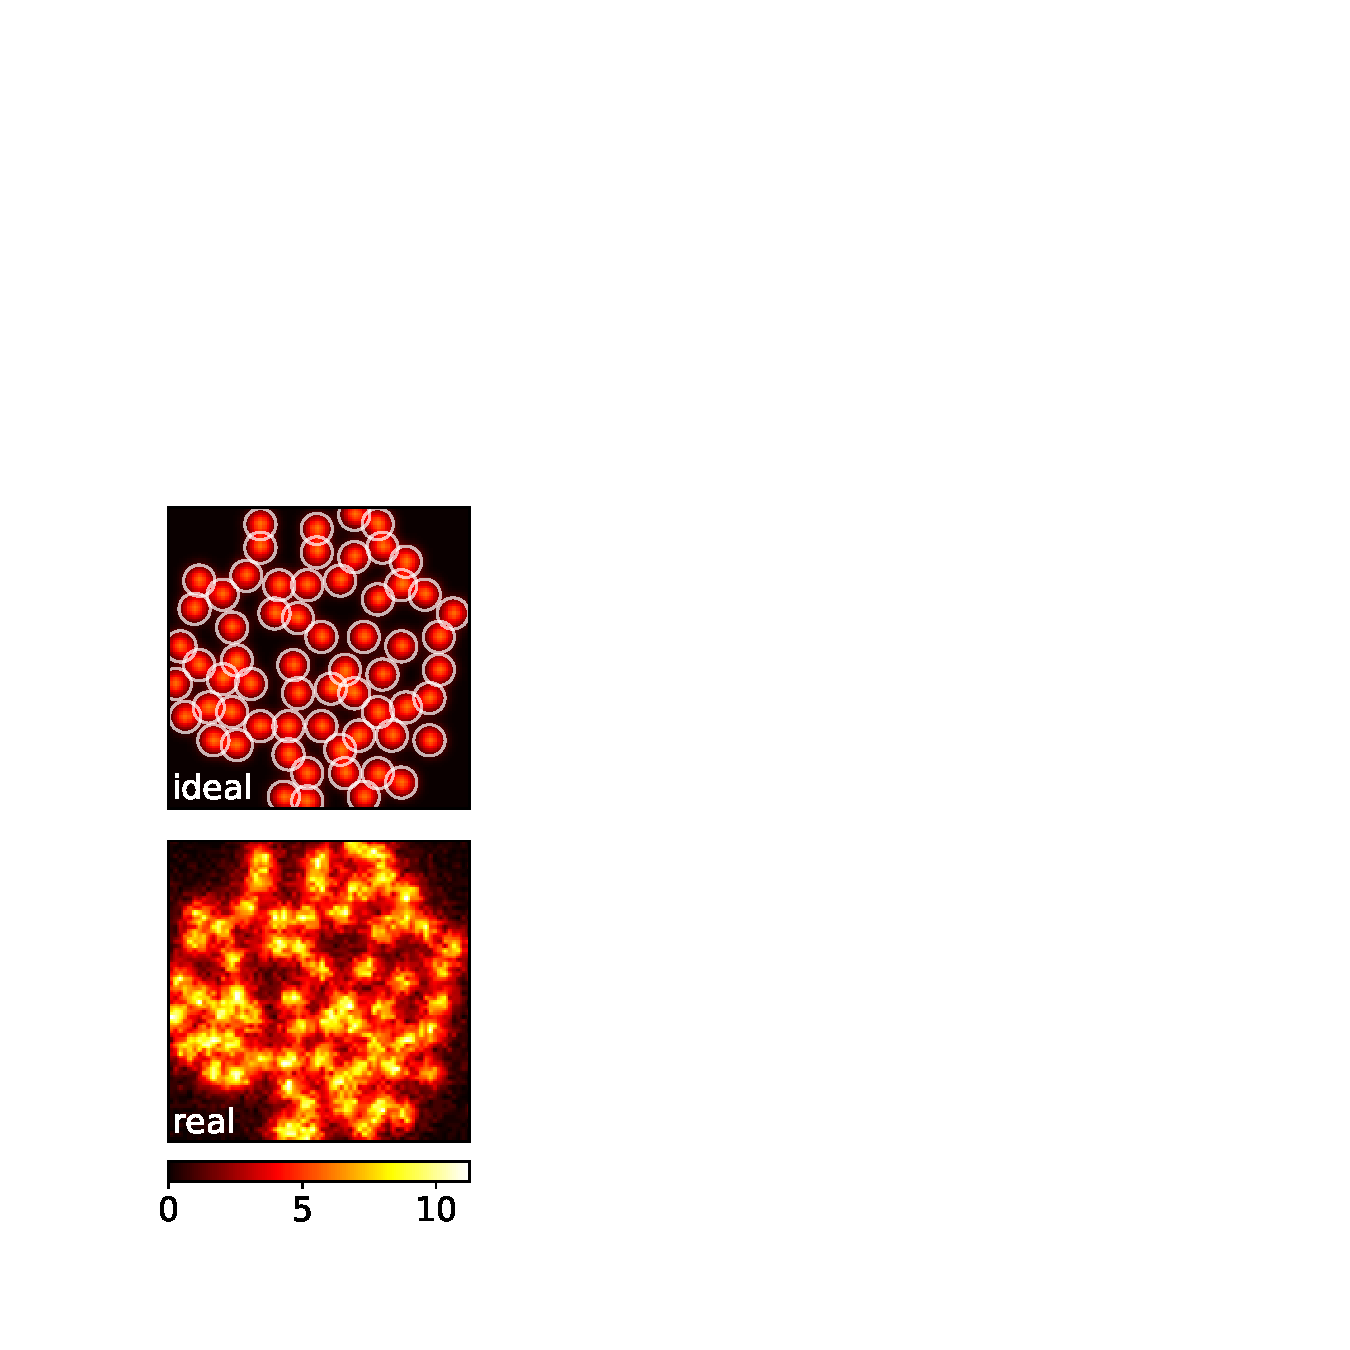
\includegraphics[scale=.5,align=t,trim=25mm 15mm 130mm 72mm, clip]{figures/regions_ideal_real.pdf}\\
    {\fontfamily{phv}\selectfont C} 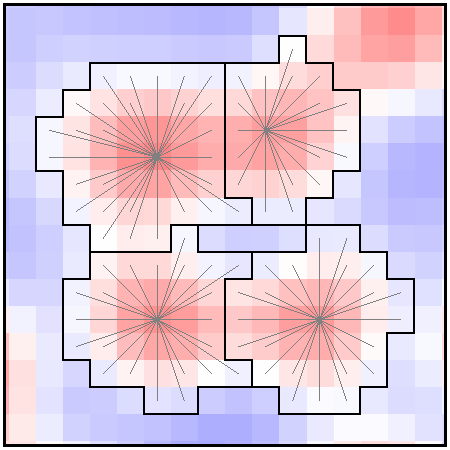
\includegraphics[scale=.33,align=t,trim={-5mm -1mm -1mm -10mm}]{figures/regions_stars.pdf}
\end{minipage}
\begin{minipage}{.6\textwidth}
    \vskip 7mm
    {\fontfamily{phv}\selectfont B} 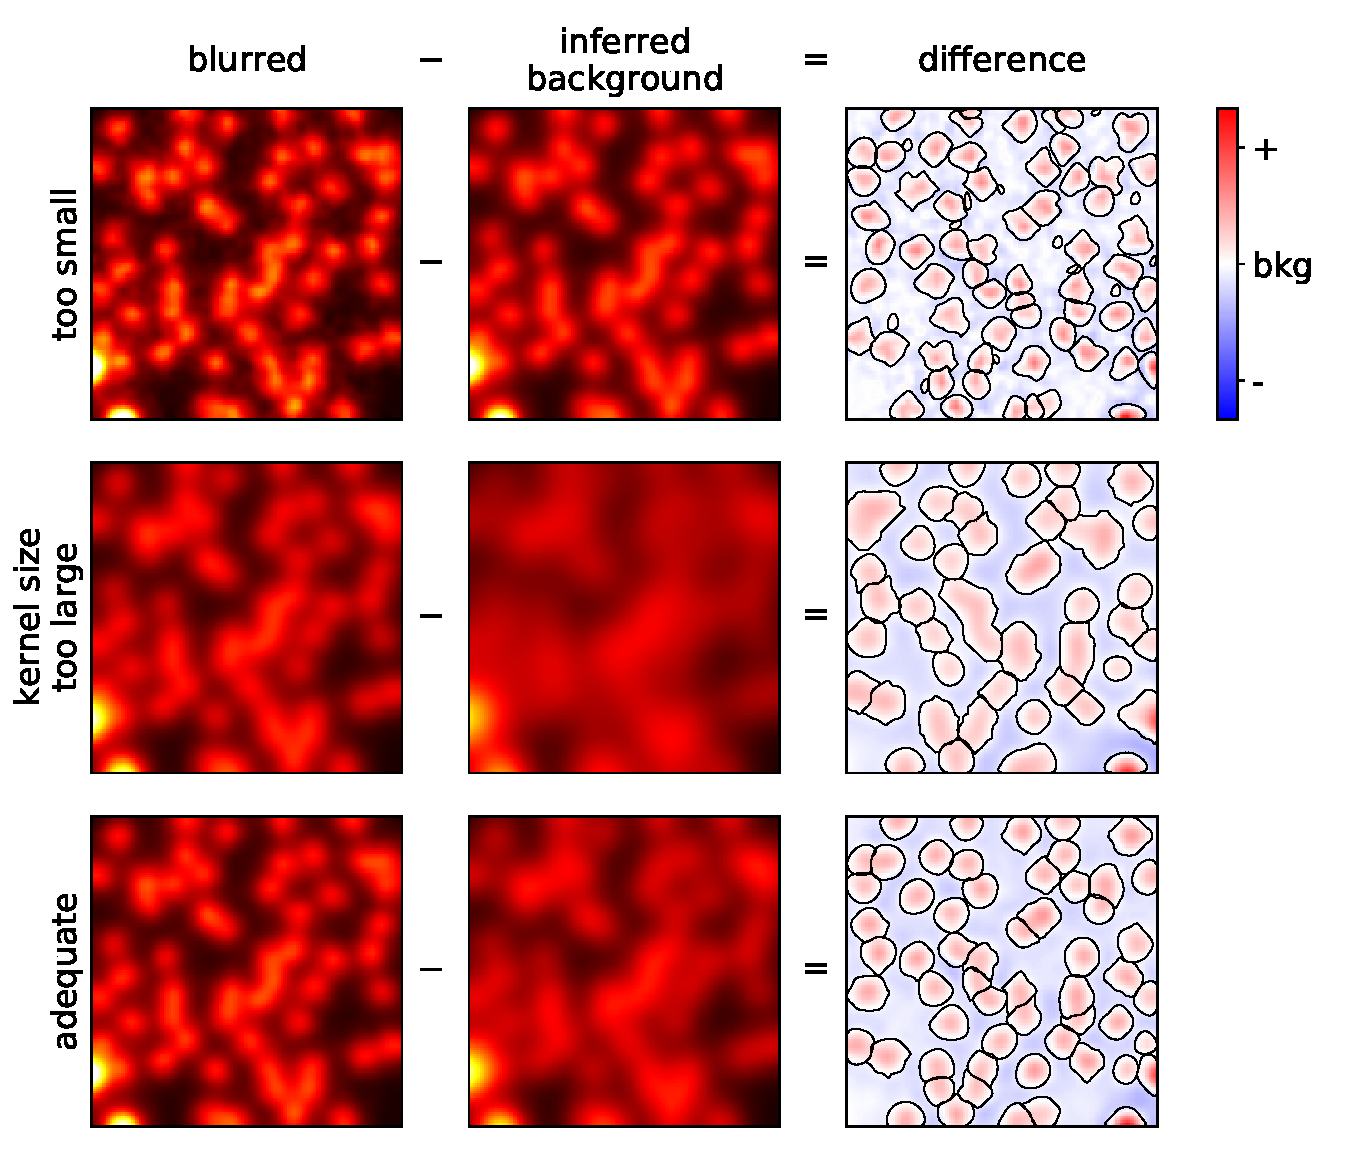
\includegraphics[scale=.5,align=t,trim=10mm 15mm 20mm 15mm, clip]{figures/regions_kernels.pdf}
\end{minipage}
\caption{
(A) Computationally created template $64{\times}64$ image with uniform spherical cells, and with Poisson noise added.
(B) Band-pass filtering of the "realistic" image from A, with different kernel sizes. The size of the kernel determines the approximate size of the ROIs obtained.
In thick red contours we emphasize misidentified ROIs; the dots indicate the real locations of the cells.
(C) Each ROI is constructed by explicitly searching for a closest peak in intensity. A pixel can only be part of a single ROI.
\label{fig:regions}}
\end{figure}

Representative image can be a mean over all frames or any other statistic.
In addition our code supports standard deviation, mean and standard deviation of the first derivative of the movie, and a ``robust maximum'' of the movie.
As "robust maximum`` we define a very high percentile of the set absolute values of a set, essentially a value close to its maximum, by default it is 10th largest. 
We avoid the maximum as a means to make analysis robust to outliers.
This statistic is sensitive to cells which fire extremely rarely during a recording, so that the mean of those pixels is negligible.
By default, we choose an average of the mean and high percentile as a representative image for band-pass filtering and ROI extraction.

\subsection{Trace processing}

\subsubsection{$z$-score and filtering}

In an ideal detector, recording a time trace of a single pixel in absence of any signal would consist of independent values of the number of photons detected during the dwell time on that pixel.
The values ($x$) are then distributed according to the Poisson distribution, with standard deviation ($\sigma_1$) being equal to the square root of the mean $\mu_1$, $\sigma_1=\sqrt{\mu_1}$.

% It is often useful to transform a set of numbers to a new 
A transformation to a new variable %$x\rightarrow z$
$$z=\frac{x-\mu}{\sigma}$$
is called {\it standard transformation}, and the new variable standard score or $z$-score (fig.\ref{fig:z_score}). Essentially, it recasts the initial quantity $x$ in the units of standard deviation from the expected mean. So, $z$ spends 95\% of the time between $-2$ and 2, and 99.7\% between -3 and 3. Probability of $z>3$ is very small $p<0.0013$, which is why it is often considered a threshold value for pointing out the outliers.
\begin{figure}[t]
    \centering
    \begin{minipage}{.49\textwidth}
        {\fontfamily{phv}\selectfont A} 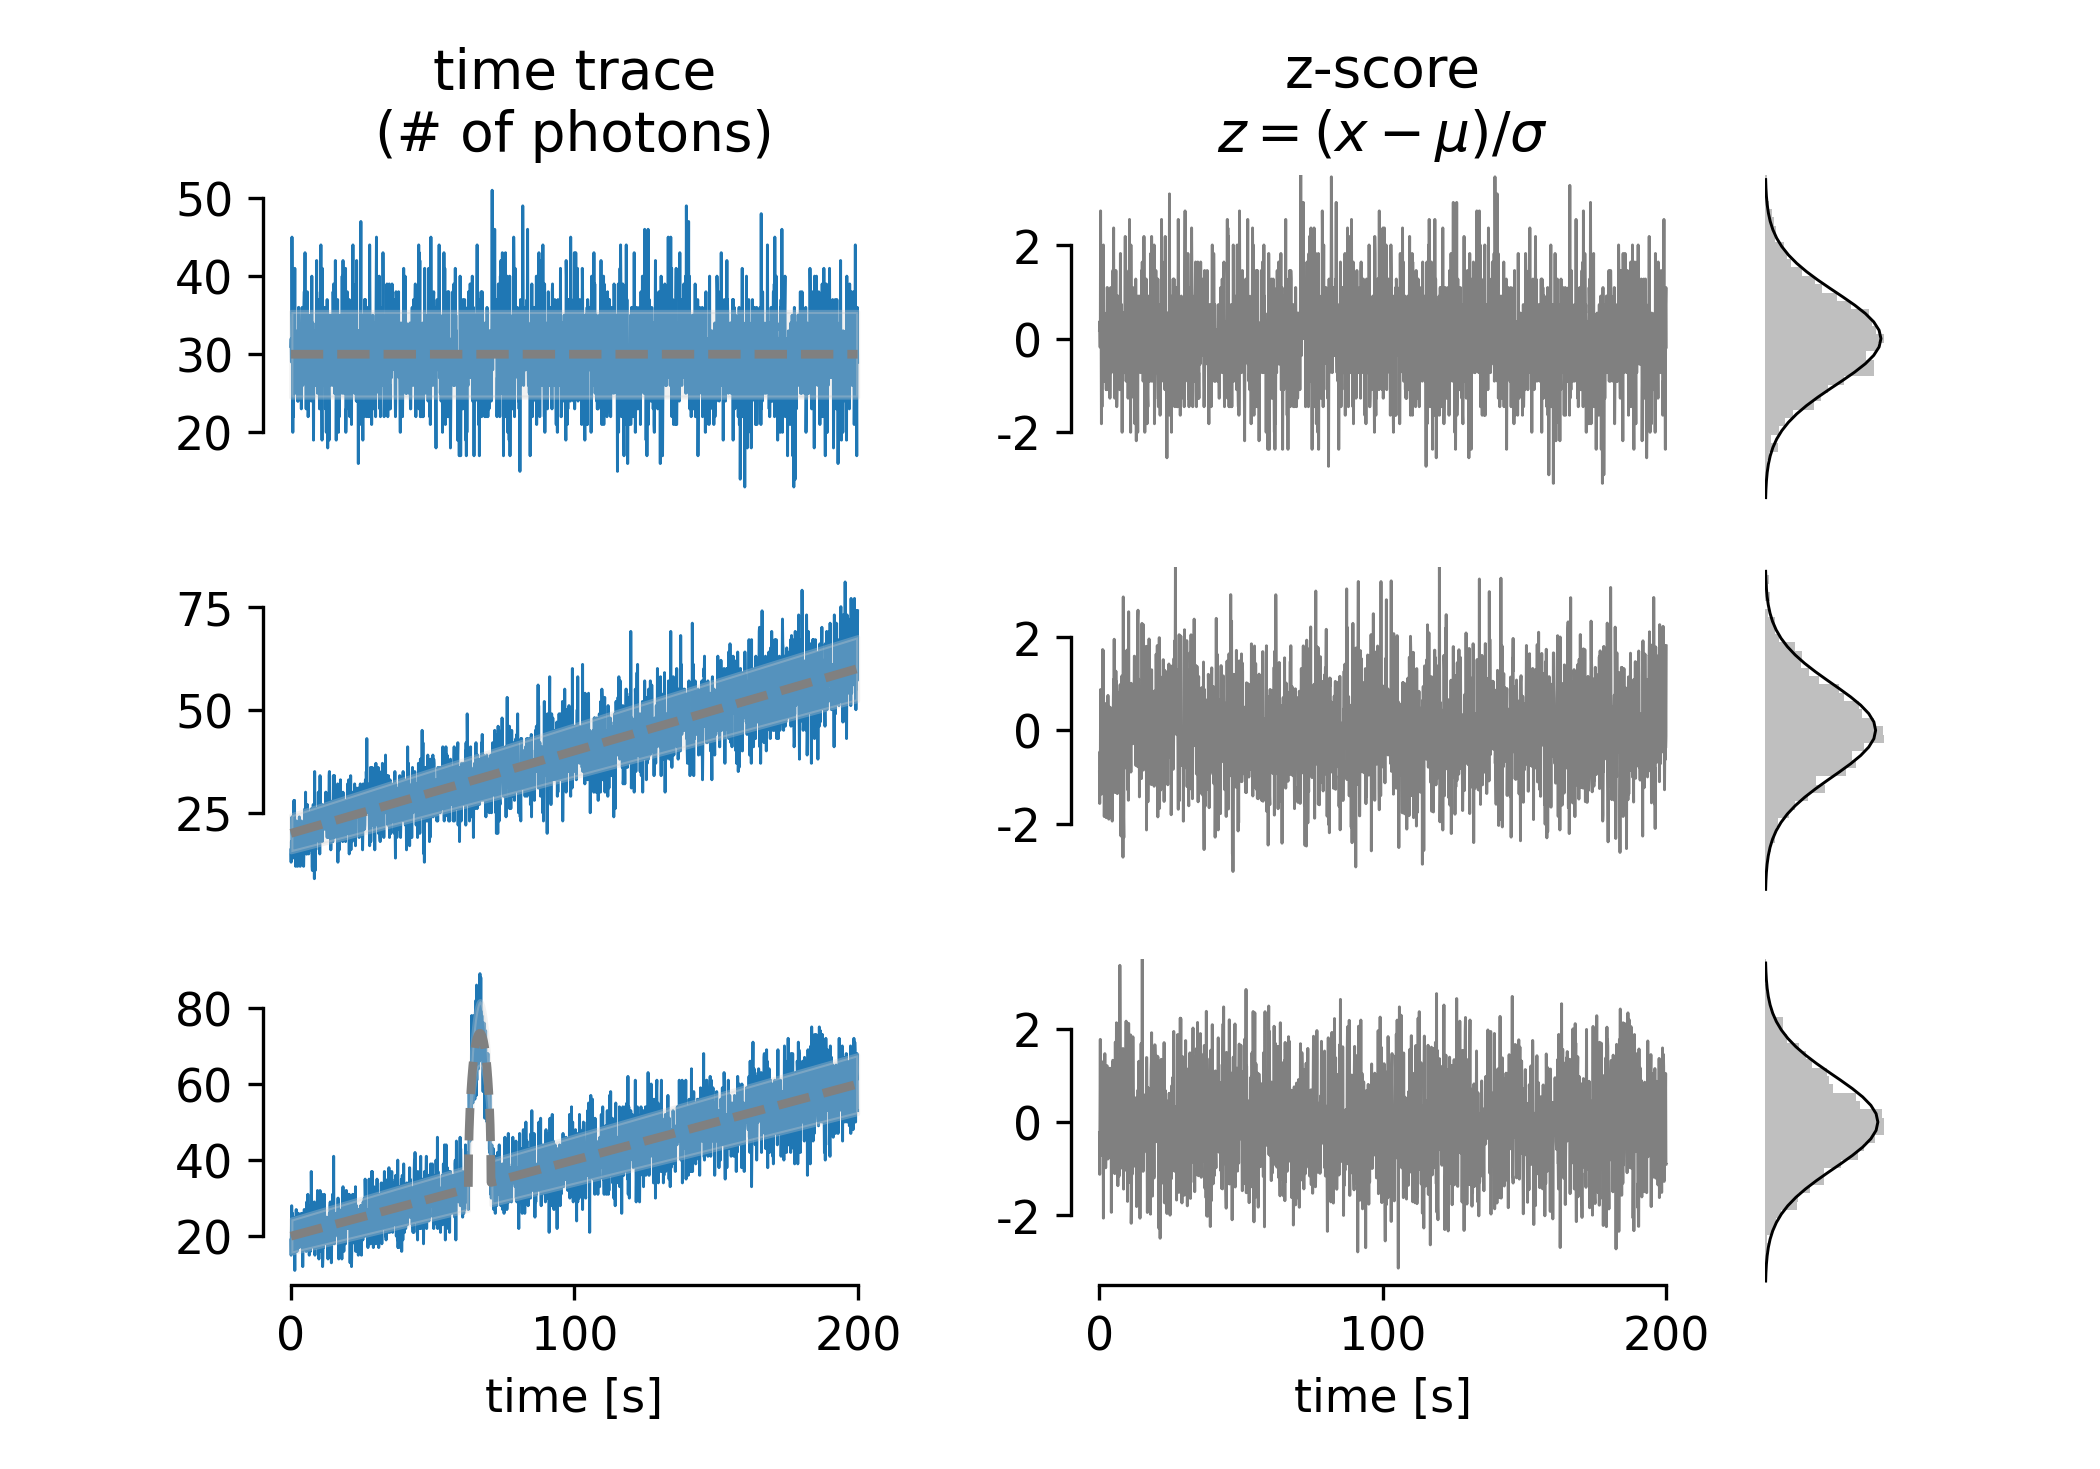
\includegraphics[scale=.5,trim=15mm 0 0 0,clip,align=t]{figures/z_score_1.png}
    \end{minipage}
    \begin{minipage}{.49\textwidth} 
        {\fontfamily{phv}\selectfont B} \includegraphics[scale=.5,trim=15mm 0mm 0 0,clip,align=t]{figures/z_score_2.pdf}
    \end{minipage}
    \caption{
    (A) \emph{Left}: Simulated traces with Poisson noise (blue) around different means (grey) with different temporal features. The shaded area represents one standard deviation interval around mean. 
    \emph{Right}: Irrespective of the shape of the mean, z-score transformation behaves exactly as a Gaussian variable with zero mean and unit standard deviation.\\
    (B) The values of s$z$-score depends on the reference. In subfigure (A), the reference curves are known, but in general they need to be inferred, typically by low-pass filtering. The cut-off frequency $f_{cut}$ of a filter determines the timescale of the events that can be detected in $z$-score. If filtered at with too high cut-off (orange), the resulting smooth curve follows too closely the trace and the event is not visible in $z$. With $f_{cut}=1/50$Hz, the resulting $z$-score has obvious outliers ($z\geq 3$), visible both in trace and in the histogram.
    \label{fig:z_score}
    }
\end{figure}

If we were to rebin a trace by a factor of $N$, the relationship between standard deviation and mean remains, but for the summed quantities $\sigma_N=\mu_N=N\mu_1$.
Normalization to the same mean as before $\tilde{\mu} = \mu_1$, results in the standard deviation $\sqrt{N}$ times lower $\tilde{\sigma} = \sigma_1/\sqrt{N}$.

Similarly, if we were to sum independent pixels ($a, b, c\dots$), 
the resulting trace would have a mean which is a simple sum of the means of individual trace, and standard deviation 
$\sigma_{a+b+\dots} = \sqrt{\mu_a+\mu_b+\dots}$. We use this when estimating the traces for ROIs, which by definition consist of multiple pixels.

\paragraph{Correcting for the filtering distortion} \lipsum[1]

\subsubsection{Realistic detectors}

means vs variance plot for photon counting and for some nikon experiment

\subsection{Identification of Events}

\newpage

\section{Analyses}
\subsection{El Toro}
\subsection{Isradipine}
\subsection{Low Ca}
\subsection{etc}

\bibliographystyle{plain}% E-Life prefers apa
\bibliography{matmet}


\end{document}
